\documentclass[final,hyperref={pdfpagelabels=false}]{beamer}
\mode<presentation>
{
  \usetheme{rc2018}
}
\usepackage[orientation=portrait,size=a0,scale=1.4,debug]{beamerposter}
\usepackage{siunitx}
\usepackage{multirow}

%%%%%%%%%%%%%%%%%%%%%%%%%%%%%%%%%%%%%%%%%%%%%%%%%%%%%%%%%%%%%%%%%%%%%%%%%%%%%%%%% 5
\title{Influence of inhibitory circuits on the frequency tuning of mitral cells}
\author[Miko]{Rebecca Miko, Christoph Metzner and Volker Steuber}
\institute{University of Hertfordshire, AL10 9AB, UK}
\date{Jul. 31th, 2018}

%%%%%%%%%%%%%%%%%%%%%%%%%%%%%%%%%%%%%%%%%%%%%%%%%%%%%%%%%%%%%%%%%%%%%%%%%%%%%%%%% 5
\begin{document}
\begin{frame}{} 
\begin{block}{Motivation}
The olfactory bulb (OB) is responsible for receiving, processing and relaying olfactory information (odours). 
Naturalistic odour stimuli have a rich temporal structure, caused by turbulent airflow.
Recent studies show that this structure contains information about the olfactory scene \cite{celani2014odor, schmuker2016exploiting}.
It has been suggested that animals might exploit this structure and extract information \cite{jacob2017olfactory}. 
Some of this information may lie in the frequency content of the stimuli \cite{schmuker2016exploiting}, therefore we studied input frequency dependent responses of mitral cells (MCs) in the OB.
Specifically, we investigated whether MCs show frequency tuning and, if they do, how different components of the glomerular layer circuitry  shape and determine the tuning.
\end{block}    

\begin{columns}[t]
\begin{column}{.48\linewidth}

\begin{block}{Model} 
\begin{figure}
\center
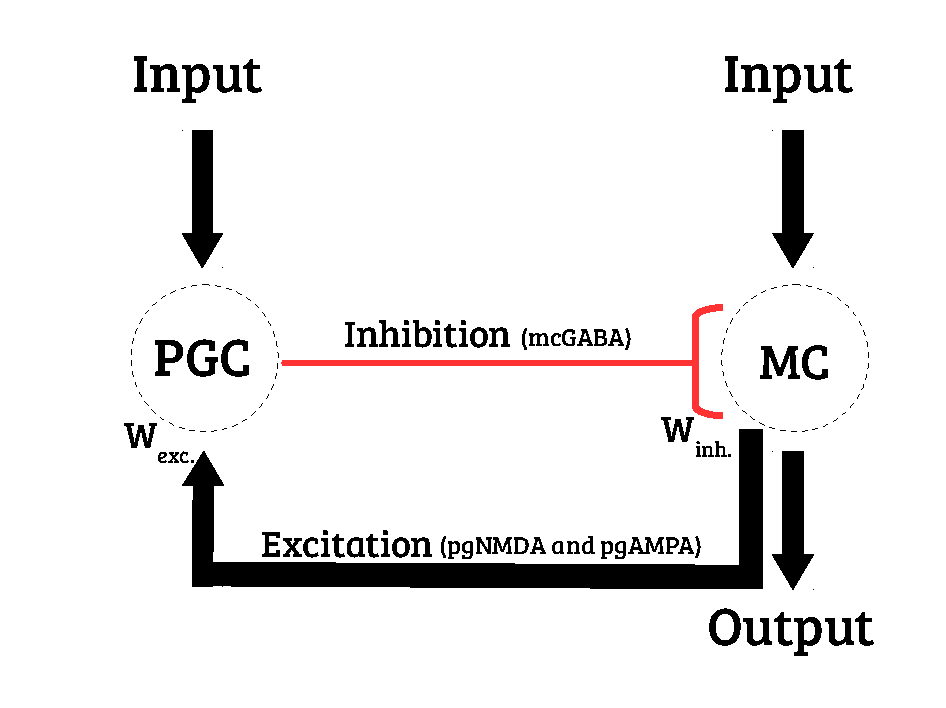
\includegraphics[scale=1.3]{poster_images/Circuit_Diagram}
\end{figure}
\begin{itemize}
\item Used a model of the OB (modified from \cite{li2013two}).
\item Modeled MC - PGC (periglomerular cells), focusing on recurrent and feed - forward inhibition in the glomerular layer.
\end{itemize}
\end{block}

\begin{block}{Method} 
\begin{figure}
\center
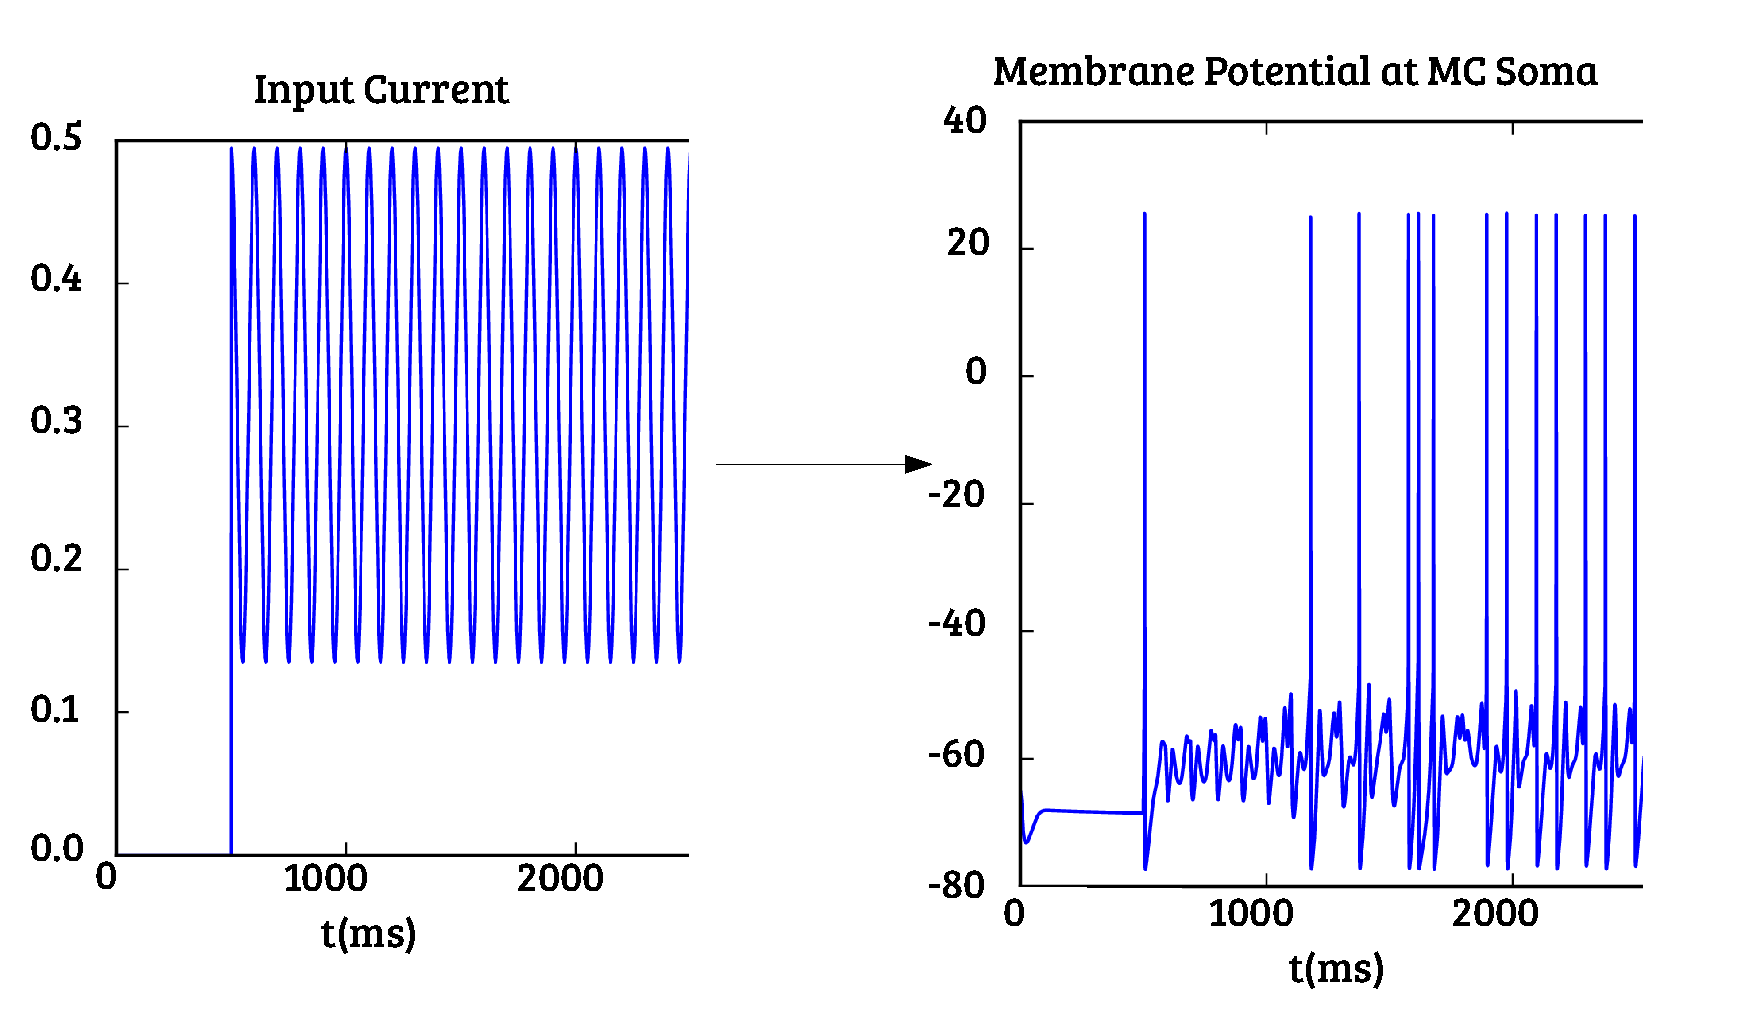
\includegraphics[scale=1]{poster_images/Figure2}
\end{figure}
\begin{itemize}
\item Used sinusoidal currents of varying frequencies as input, using the equation:
\[
\text{y(t) = c\cdot sin(2} \cdot\pi\cdot\text{ft +} \varphi\text{) + 0.18}
\]
\item Where strength of input to MC (c) = 0.45nA and phase ($\varphi$) = 0.
\end{itemize}

\begin{center}
\begin{tabular}{ |c| c c c c c | }
\hline 
\multirow{2}{12em}{\centering Parameter} & \multicolumn{5}{|c|}{\multirow{2}{*}{\centering Iteration Values}}\\
\multirow{2}{*}{} & \multirow{2}{*}{} & \multirow{2}{*}{} & \multirow{2}{*}{} & \multirow{2}{*}{} & \multirow{2}{*}{}\\
\hline
\multirow{2}{12em}{\centering PGC Input Strength (i\cdot c)} & \multirow{2}{*}{0.2} & \multirow{2}{*}{0.3} & \multirow{2}{*}{0.4} & \multirow{2}{*}{0.5} & \multirow{2}{*}{0.6} \\ 
\multirow{2}{*}{} & \multirow{2}{*}{} & \multirow{2}{*}{} & \multirow{2}{*}{} & \multirow{2}{*}{} & \multirow{2}{*}{}\\
\hline
\multirow{2}{12em}{\centering MC - PGC excitation strength (\mbox{$\text{W}_{\text{exc}}$})} & \multirow{2}{*}{2.0} & \multirow{2}{*}{4.0} & \multirow{2}{*}{6.0} & \multirow{2}{*}{8.0} & \multirow{2}{*}{10.0}  \\
\multirow{2}{*}{} & \multirow{2}{*}{} & \multirow{2}{*}{} & \multirow{2}{*}{} & \multirow{2}{*}{} & \multirow{2}{*}{}\\
\hline
\multirow{2}{12em}{\centering PGC - MC inhibition strength (\mbox{$\text{W}_{\text{inh}}$})} & \multirow{2}{*}{1.0} & \multirow{2}{*}{2.0} & \multirow{2}{*}{3.0} & \multirow{2}{*}{4.0} & \multirow{2}{*}{5.0} \\
\multirow{2}{*}{} & \multirow{2}{*}{} & \multirow{2}{*}{} & \multirow{2}{*}{} & \multirow{2}{*}{} & \multirow{2}{*}{}\\
\hline
\multirow{2}{12em}{\centering Frequency (f)} & \multirow{2}{*}{1.0,} & \multirow{2}{*}{2.0,} & \multirow{2}{*}{3.0,} & \multirow{2}{*}{... ,} & \multirow{2}{*}{40.0}\\
\multirow{2}{*}{} & \multirow{2}{*}{} & \multirow{2}{*}{} & \multirow{2}{*}{} & \multirow{2}{*}{} & \multirow{2}{*}{}\\
\hline
\end{tabular}
\end{center}

\begin{itemize}
\item Parameter combinations: PGC input strength, MC - PGC excitation strength and PGC - MC inhibition strength.
\item Constructed frequency tuning curves and then extracted the peak resonance frequency (fig 3).
\item Extracted the resonance strength of the tuning Q (fig 3), measured as:
\[
\text{Q =} \frac{\text{(F}_{\text{max}} \text{ - F}_{\text{min}}\text{)}}{<\text{F}>}
\]
\item \mbox{$\text{F}_{\text{max}}$} and \mbox{$\text{F}_{\text{min}}$} is maximum and minimum firing rate.
\item $<$F$>$ is mean firing rate over all measured frequencies.
\end{itemize}
\end{block}

\end{column}
\begin{column}{.48\linewidth}

\begin{block}{Results}
\begin{figure}
\center
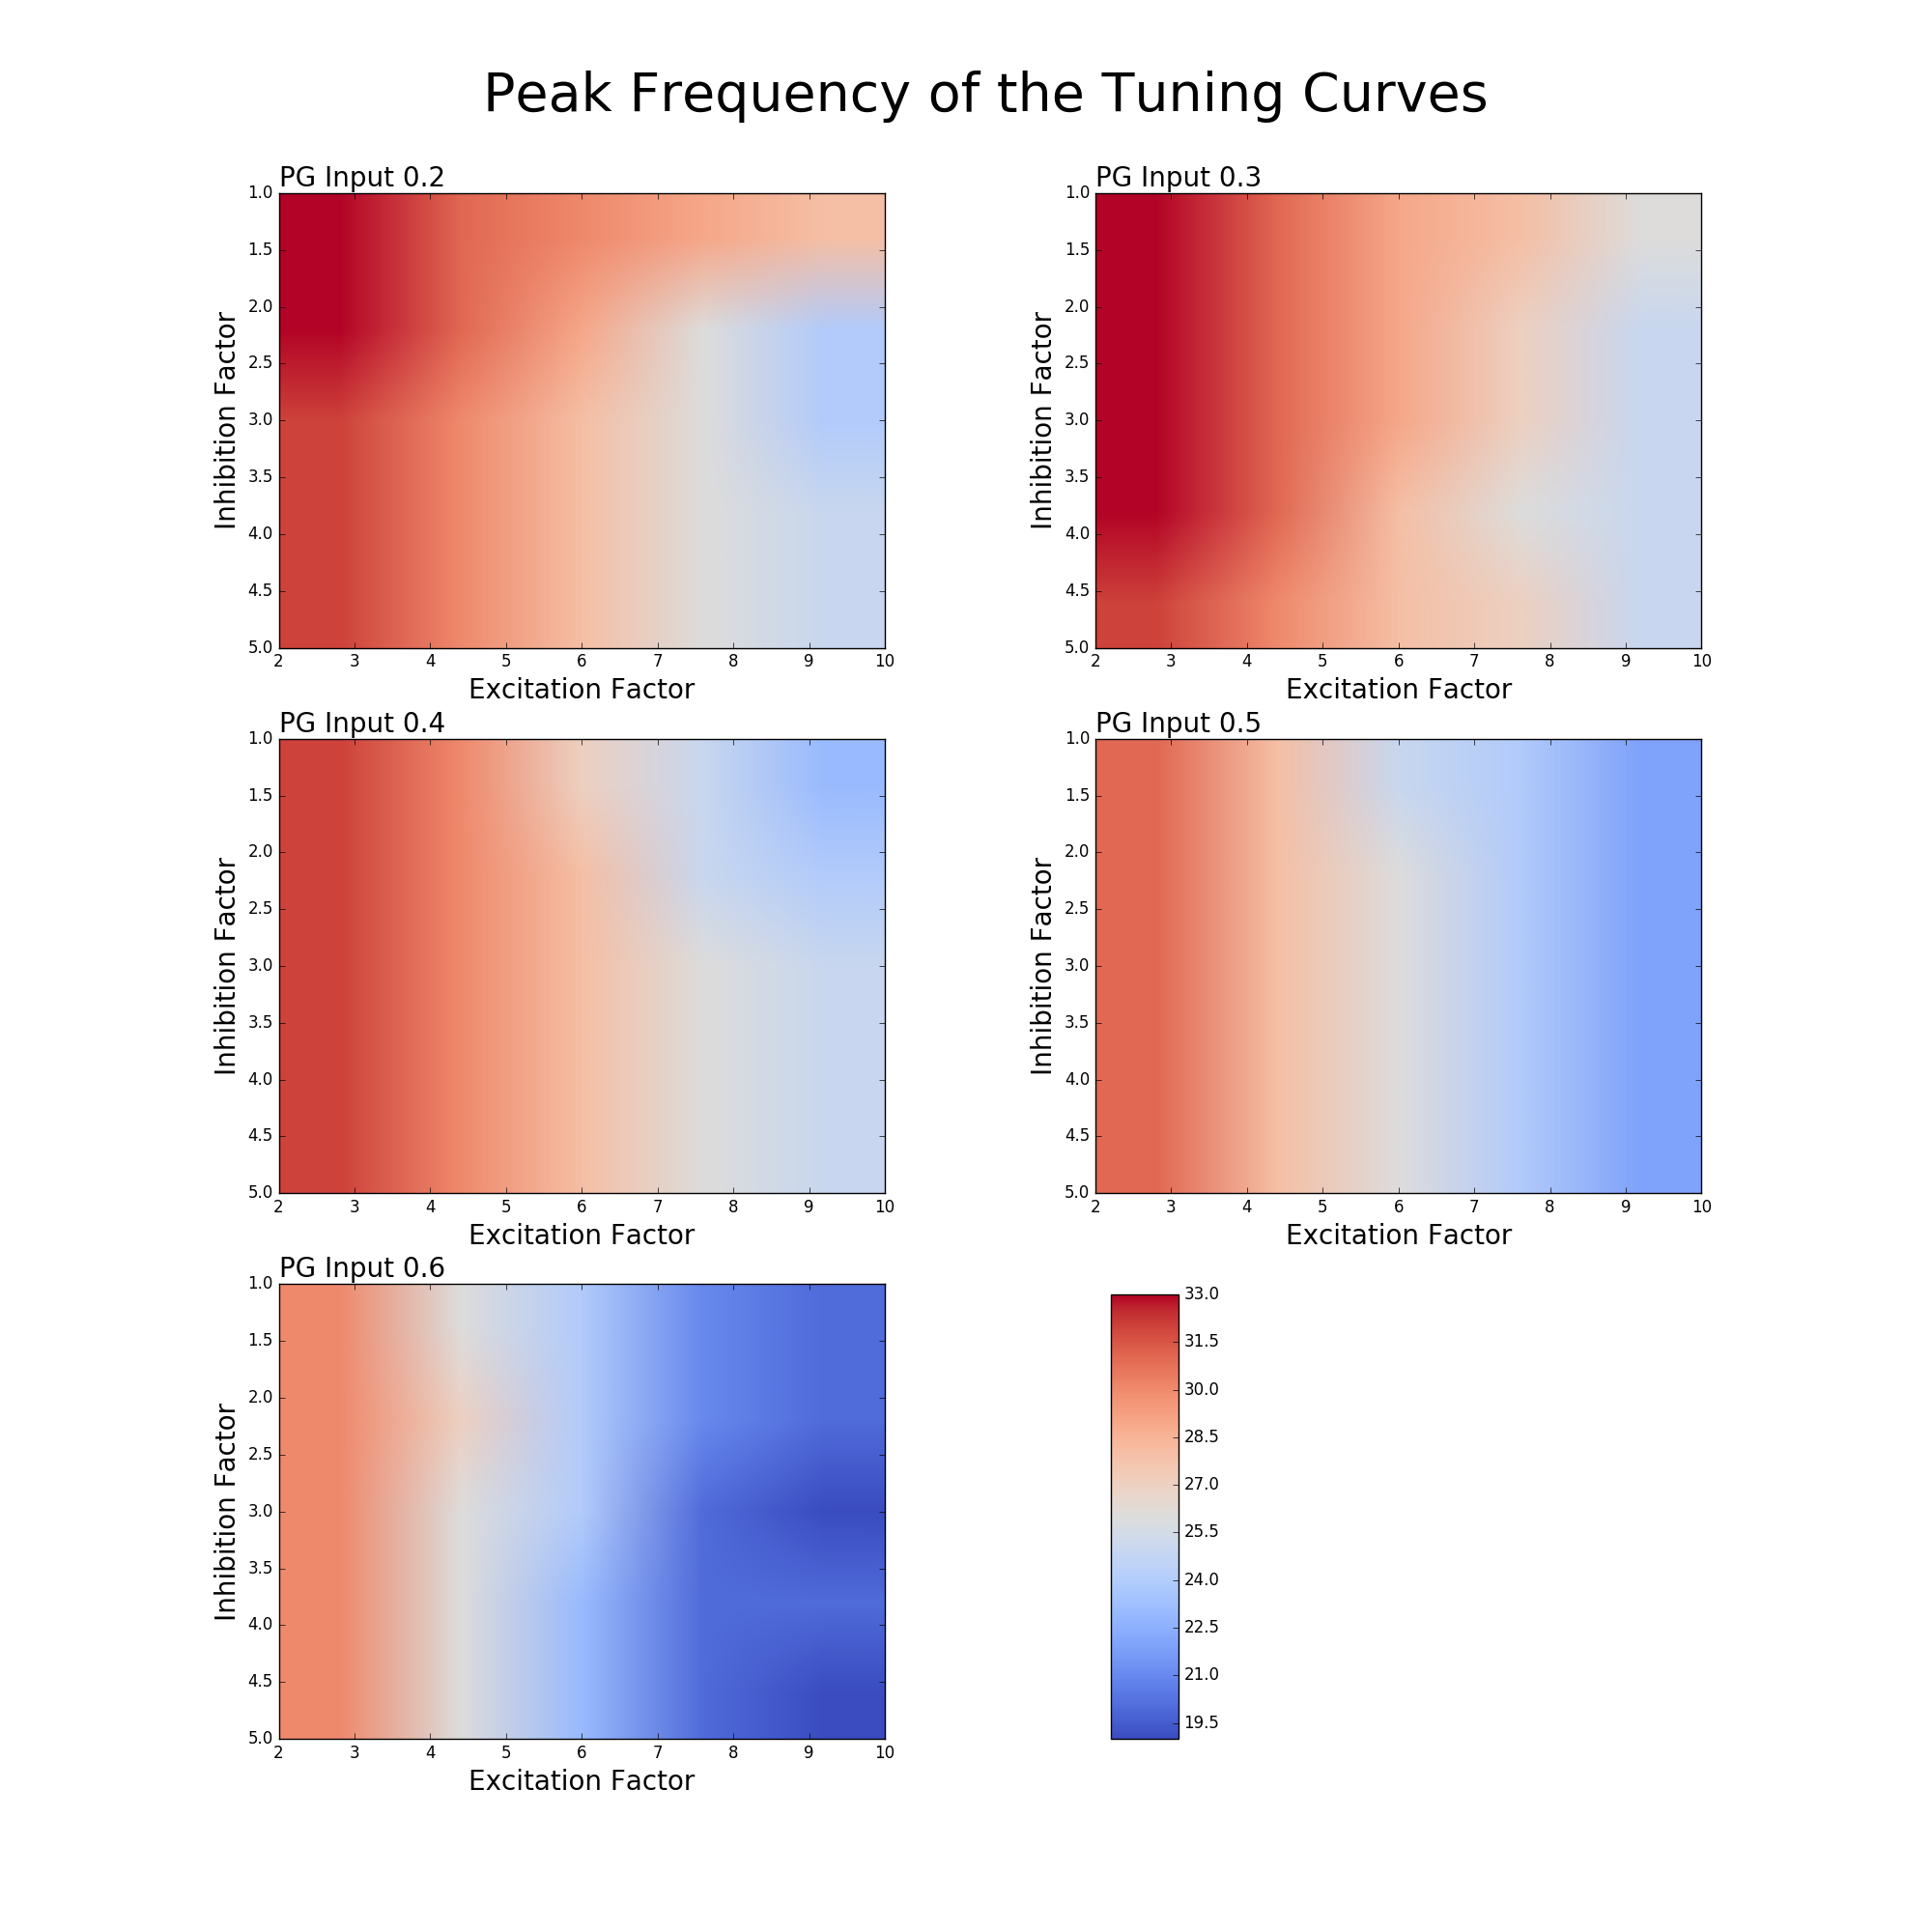
\includegraphics[scale=0.55]{poster_images/Contour_plot_tuning_frequency}
\end{figure}

\begin{itemize}
\item Resonance frequency decreased as the excitation of the PGC increased (both from input and the MC).
\item Strength of PGC inhibition onto the MC did not have a strong effect.

\begin{figure}
\center
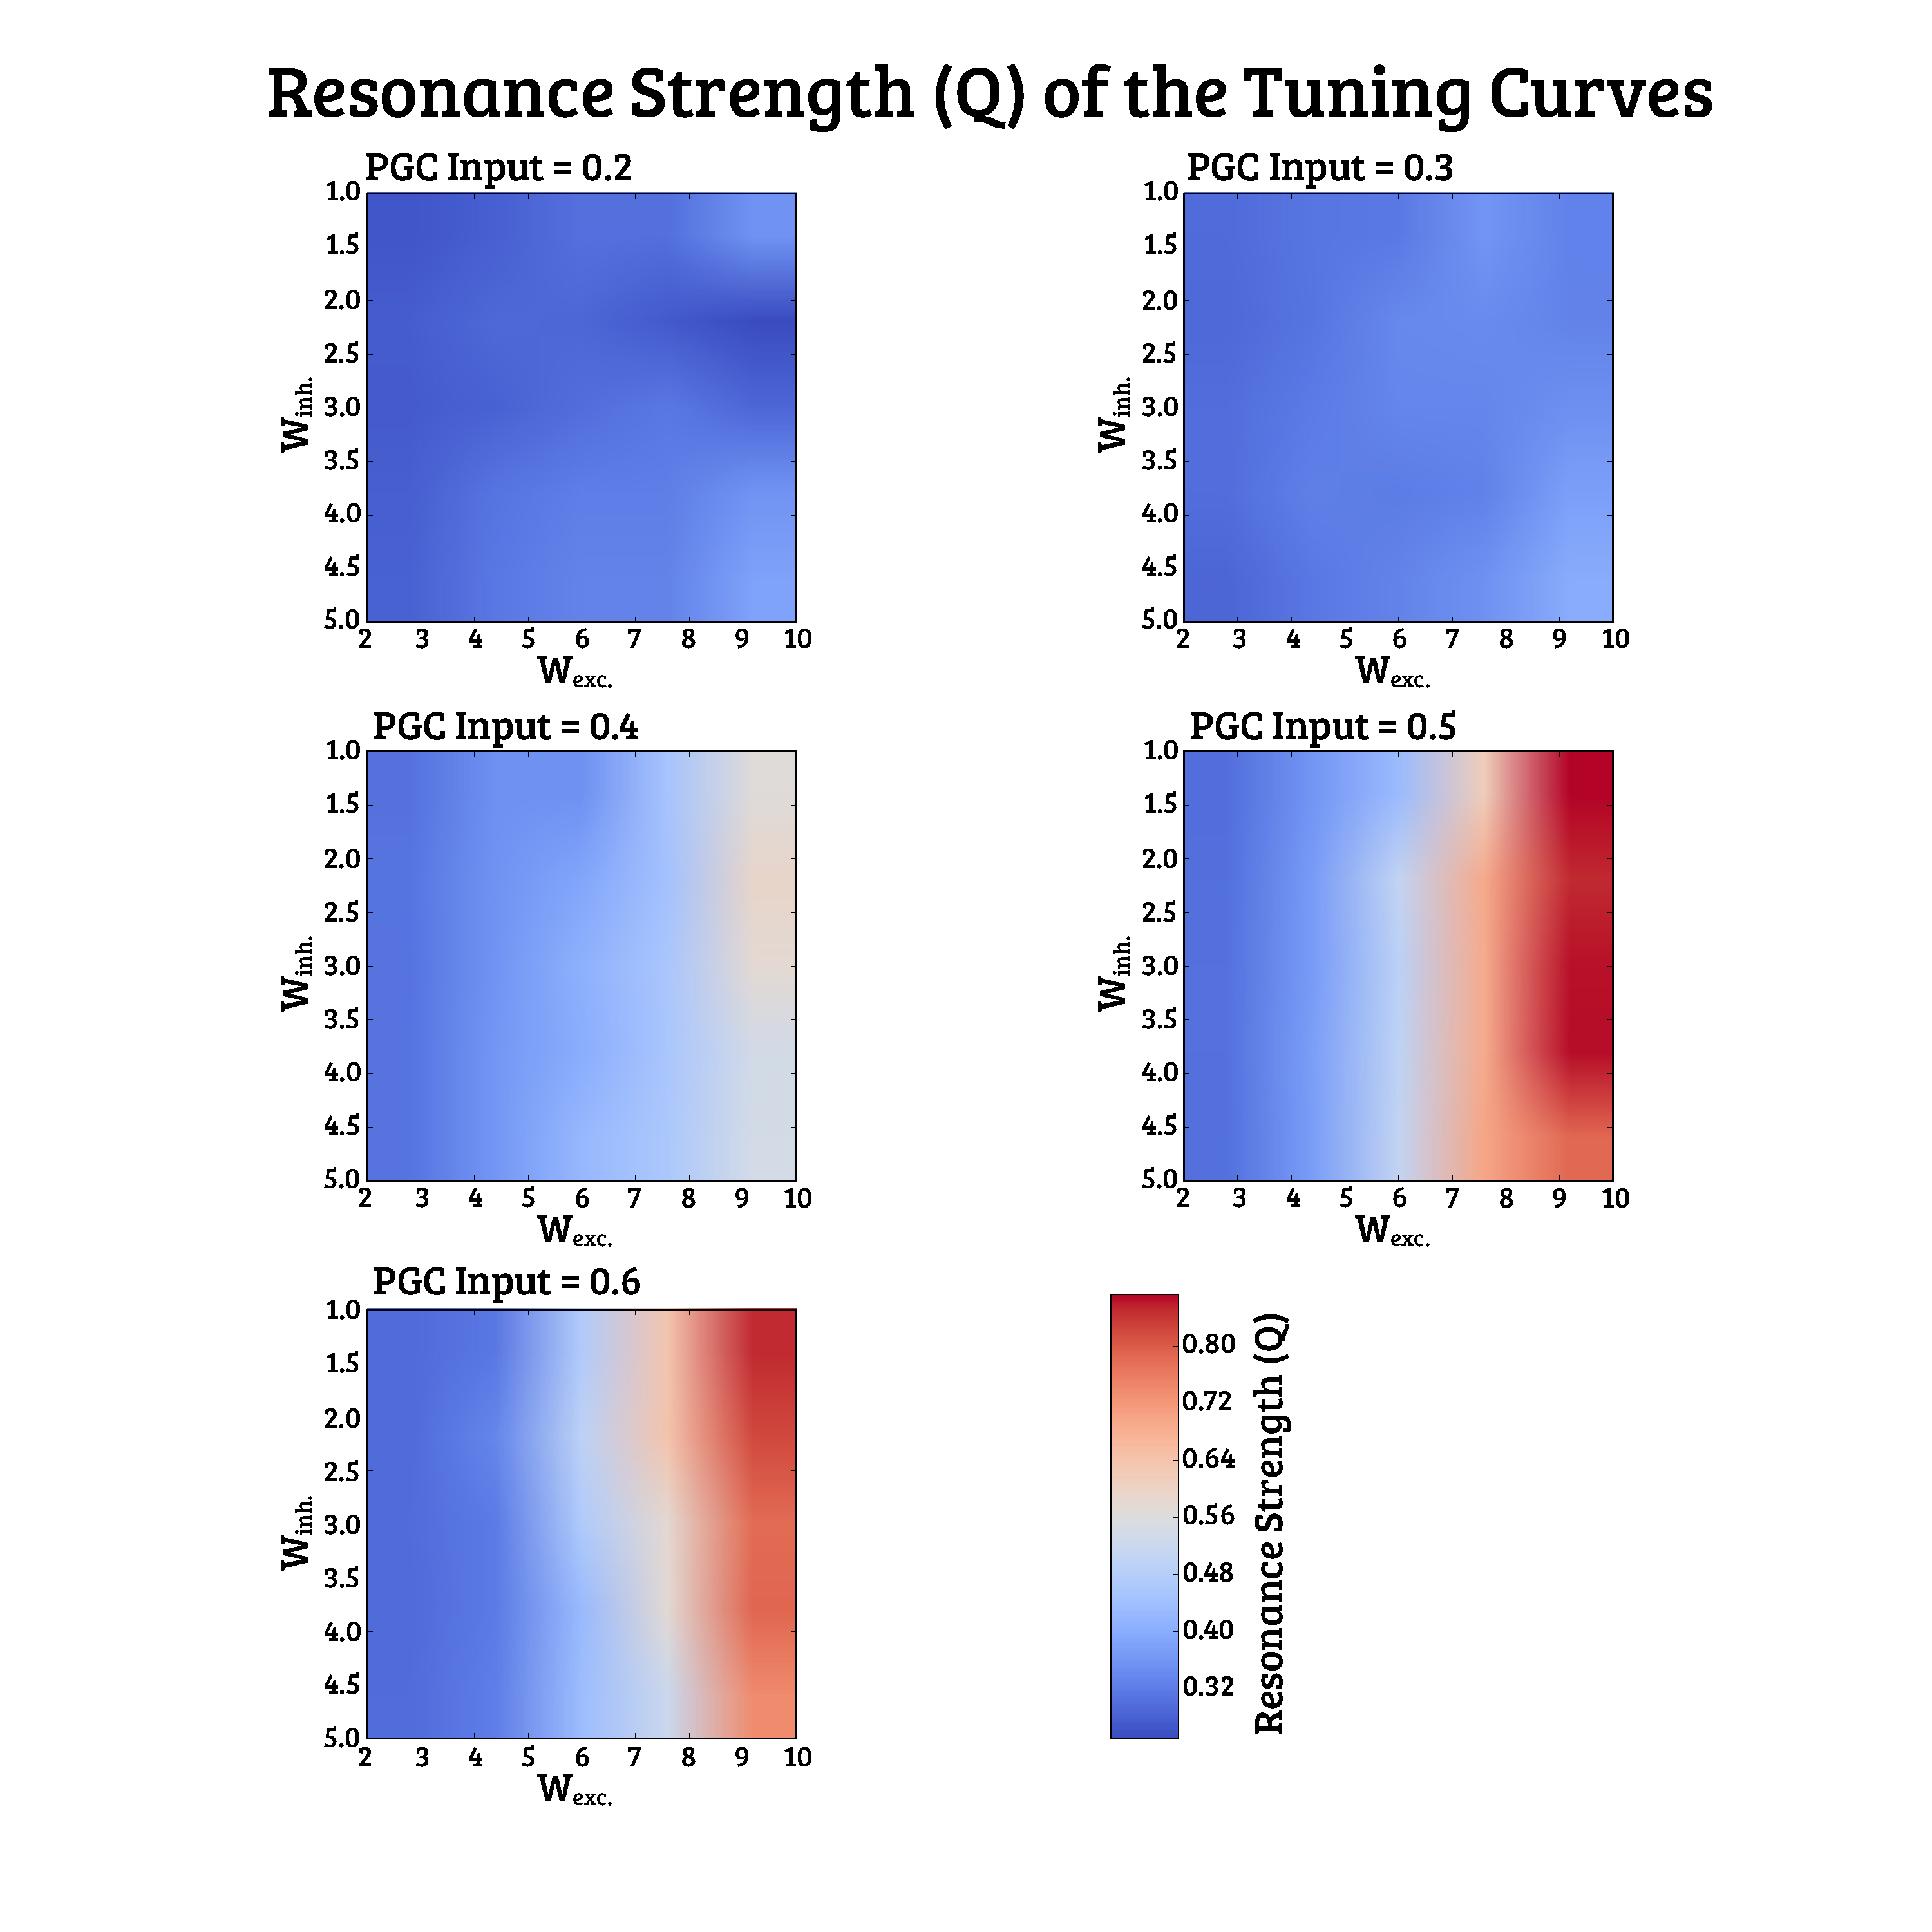
\includegraphics[scale=0.55]{poster_images/Contour_plot_tuning_strength}
\end{figure} 

\item Resonance strength increased with the strength of the excitatory connection, when the PGC received sufficient external input.
\end{itemize}
\end{block}

\begin{block}{Discussion}
\begin{itemize}
\item Results suggest the MC can show frequency tuning.
\item Therefore, the OB might be able to detect the frequency composition of signals.
\item This could be used for olfactory scene analysis.
\item However, we only see tuning in a narrow frequency range.
\end{itemize}
\end{block}

\begin{block}{References}
\nocite{*}
\bibliographystyle{acm}
{\footnotesize
\bibliography{BibList}}
\end{block}

\end{column}
\end{columns}
\end{frame}
\end{document}

%%%%%%%%%%%%%%%%%%%%%%%%%%%%%%%%%%%%%%%%%%%%%%%%%%%%%%%%%%%%%%%%%%%%%%
